
\documentclass[a4paper]{article}

\usepackage{hyperref}
%\hypersetup{
%colorlinks=false,              % bool: Liens colorés
%pdfborder={0 0 0}             % Ne pas encadrer les liens
%}
\usepackage[utf8]{inputenc}  
\usepackage[francais]{babel}  
\usepackage[top=2cm, bottom=2cm, left=2cm, right=2cm]{geometry}
\usepackage{graphicx}
\usepackage[final]{pdfpages} 
\usepackage{rotating}
\usepackage{eurosym}
\usepackage{lscape}
\usepackage{float}
% définir les commandes ici

% s'il y a beaucoup de commandes et de packages à inclure n'h&ésitez pas
% à mettre tout ça dans un fichier include.tex et l'inclure
% \input{include.tex}


\begin{document}

%------------------------------------- Page de titre
\begin{titlepage}
~ 
\vfill
	\begin{center}
		\begin{Huge}
		SOA : Dossier d'architecture technique\\
		\end{Huge} 
\vfill
		\textbf{Hexanome 4211 :} 
		\\Sandra \bsc{Mondain}, Elisa \bsc{Abidh}, 
		\\Gaël \bsc{Motte}, Armand \bsc{Rossius}, 
		\\Rémi \bsc{Fradet}, Nicolas \bsc{Silva}, Julien \bsc{Levesy}\\

\vfill		
		\begin{Large}
		Avril 2011
		\end{Large}
\vfill

	\end{center}
\vfill
\end{titlepage}
%----------------------------------------------------

%--------------------------------- Table des matières
\newpage
\tableofcontents
\newpage
%----------------------------------------------- Plan

\section{Introduction}

Ce dossier clarifie l'architecture du système d'information au niveau technique, c'est à dire comment le système est mis en place ce qui concerne l'architecture réseau des agences, la communication entre agence et la topologie des bases de données du système global. 

\section{Architecture technique du SI}

%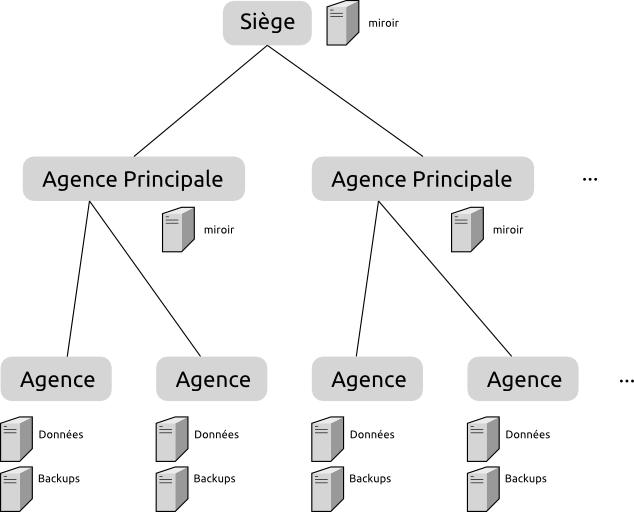
\includegraphics{archi_base.png}

L'architecture du nouveau système d'information doit offrir une visibilité dans toutes les agences à un grand nombre de données partagées. Cette visibilité doit être à la fois performante et cohérente, c'est à dire que les réponses à une même requête effectuée depuis différentes agences doivent être identiques.

\subsection{Architecture du système au niveau agence}

Chaque agence possède un réseau placé derrière un pare-feu, comprenant deux sous-réseaux.
\begin{itemize}
  \item Le premier sous-réseau est placé en dessous d'un routeur VPN, créant ainsi un réseau virtuel global et sécurisé, sur lequel sont échangées les informations entre agences. Les bases de données ainsi que les postes de travail des agents sont également placés dans ce sous-réseau.
  \item Le second sous-réseau comprend, si besoin, les services dont la sécurité est plus difficile à assurer. Il est en effet important ne pas placer, par exemple, un service web ouvert aux clients de la banque, très susceptible d'essuyer des attaques sur le même sous-réseau que les bases de données comportant des informations confidentielles ou organisationnelles. 
\end{itemize}

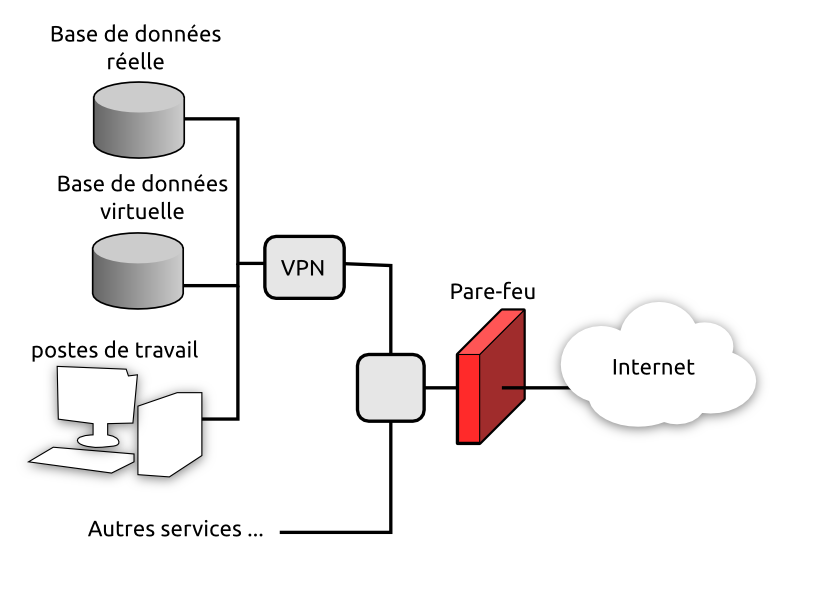
\includegraphics[width=\linewidth]{Includes/archi_agence.png}


\subsection{Architecture du système au niveau national}
\subsubsection{ Stockage des données }

Les données sont réparties en fonction de leur nature :
\begin{itemize}
  \item Les informations clients sont centralisées au siège de l'entreprise.
  \item Les agendas ainsi que les contacts sont répartis entre les agences principales de sorte que les agences principales conservent les données relatives à leurs agences affiliées.
\end{itemize}
  
\subsubsection{ Flux de données }


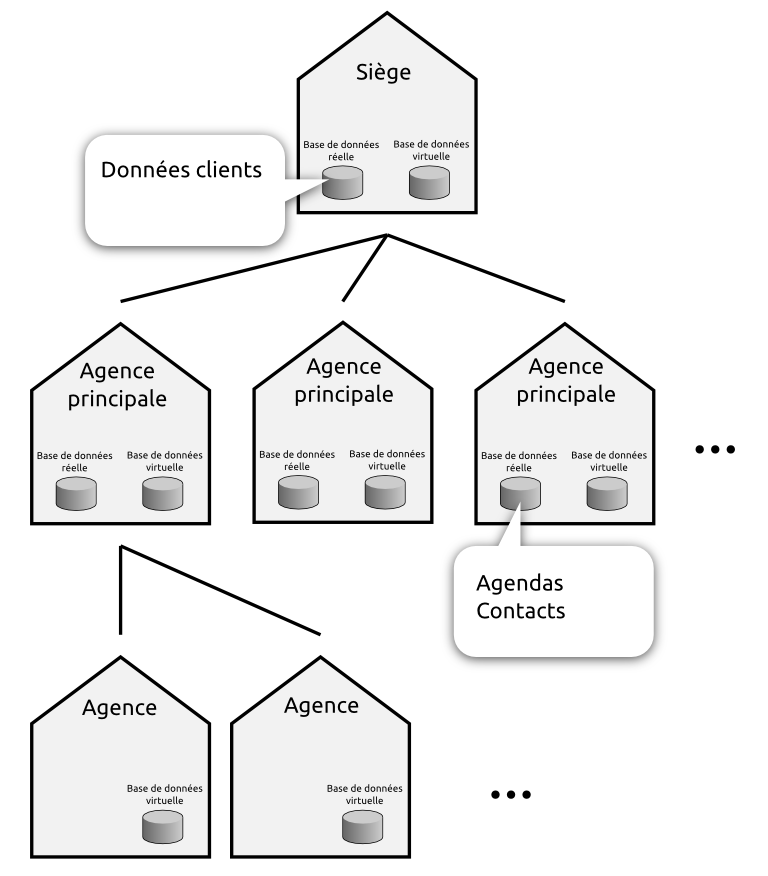
\includegraphics[width=\linewidth]{Includes/arch_hierarchie.png}


Les postes de travail, notamment ceux des agents, sont placés sur le réseau VPN global et peuvent ainsi interroger les serveurs de données à distance, au travers des applications de gestion des éléments du SI. Toutes les informations stockées sur les serveurs de données sont versionnées sur plusieurs mois. Chaque agence possède une \textit{base de donnée virtuelle} qu'interrogent les applications des employés.\\
Une base de donnée virtuelle est un programme qui interroge les serveurs de données (locaux ou distants) afin de répondre aux requêtes du personnel, et conserve temporairement les informations de ces requêtes. Ce système permet d'abstraire l'interrogation des bases de données physiques, afin que les couches applicatives supérieures n'aient pas à se soucier de la localisation des serveurs de données, et fournit un accès plus rapide aux données en évitant de surcharger le réseau. En effet, les informations temporairement conservées permettent à la base de donnée virtuelle d'éviter certains transferts de données volumineux sur le réseau si les données sont déjà présentes localement suite à une requête similaire. Afin de savoir si les informations locales sont à jour, les bases de données virtuelles comparent l'identifiant de version des données locales à l'identifiant de version des données du serveur distant.\\
Le schéma ci-dessous montre l'accès aux données par un poste situé dans une agence A. Les données recherchées peuvent être stockées soit sur un serveur local, soit sur un serveur d'une autre agence (B), soit dans la mémoire temporaire de la base de données virtuelle. \\
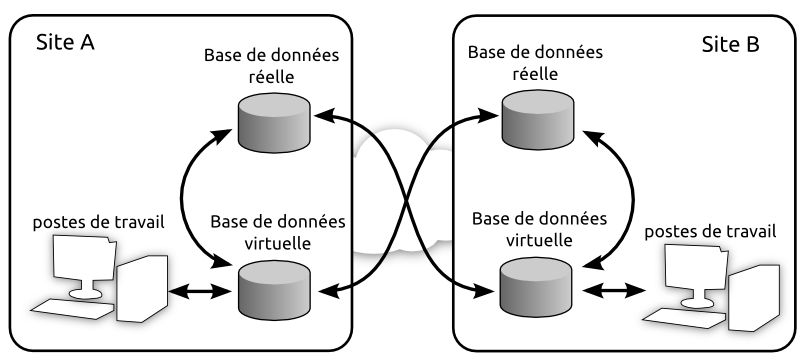
\includegraphics[width=\linewidth]{Includes/archi_bddVirtuelle.png}

~\\
Ainsi, les requêtes d'accès et de modification des données passent par les application de virtualisation de bases de données qui fournissent une interface unifiée, simplifiée et transparentes à toutes les agences.


\end{document}
